\documentclass{article}

% Language setting
% Replace `english' with e.g. `spanish' to change the document language
\usepackage[english]{babel}

% Set page size and margins
% Replace `letterpaper' with`a4paper' for UK/EU standard size
\usepackage[letterpaper,top=2cm,bottom=2cm,left=3cm,right=3cm,marginparwidth=1.75cm]{geometry}

% Useful packages
\usepackage{amsmath}
\usepackage{graphicx}
\usepackage[colorlinks=true, allcolors=blue]{hyperref}
\usepackage[numbers]{natbib}

\title{Human-AI interactions analysis}
\author{Anna Ferrari, Tommaso Ballarini, Walter Scafa}

\begin{document}
\maketitle

\begin{Keywords}
Human-AI interactions; Conversational system; Social Chatbot; Artificial intelligence; Replika
\end{Keywords}


\section{Introduction}

Building machines able to converse with humans using natural language has been the fundamental challenge in the field of Artificial Intelligence (AI) from the earliest stage of its development. Inspired by the Turing test, whose goal was to determine whether a machine could exhibit intelligent behavior indistinguishable from that of a human by assessing its ability to engage in natural conversations \cite{turing1950computing}, multiple researchers made an attempt to create "social chatbots" (SC), i.e., computer programs capable of convincingly conducting a human-like conversation using audio or text \cite{article}. 
While early chatbots engage in simple chitchat, advances in Large Language Models (LLMs) have enabled AI chatbots to generate contextually appropriate responses, understand not only the literal meaning of words but also how expressions can convey meanings different from their individual words, and recognize and track the user’s emotional state \cite{chu2025illusionsintimacyemotionalattachment, article}. 
As computers became increasingly capable of mimicking human behavior (displaying personality, expressing empathy, and tracking users’ emotional states) a new field emerged at the intersection of AI, ethics, and sociology. This field investigates whether human–computer interactions can be analyzed using sociological paradigms and approaches traditionally applied to human relationships \cite{inproceedings}. In 1994, the publication of Computers are Social Actors by C. Nass, J. Steuer, and E. R. Tauber introduced the so-called "CASA paradigm," which posits that people respond to computers in fundamentally social ways, applying the same rules, norms, and expectations that govern interpersonal relationships \cite{10.1145/259963.260288,article}. This work laid the foundation for applying theories of human interaction to human–machine relationships and opened the way for a broad scholarly discourse on AI companionship, along with the social and psychological issues it raises. Previous literature studying SC attempted to analyze the phenomenon using existing theories, such as the Social Response Theory, Social Penetration Theory and the Attachment Theory \cite{inproceedings, article1, article2}, but lacked in explaining the underlying mechanisms of AI that facilitate the creation of personal relationships with SC.  Indeed, vast majority of research in this field has relied on self-reported surveys, small-scale qualitative studies and focus-group interviews. This paper makes an attempt to contribute to the discourse by leveraging methods from computational social science to analyze large-scale text-based interactions between Reddit users who share experiences of AI companions and different SC. 
Specifically, we examine over 30,000 user-shared conversations from Reddit communities (Replika, MyBoyfriendIsAI, AIRelationship...), combining computational text-analysis, topic modeling and emotion detection to investigate more deeply the interplay between algorithmic design and human behavior. 
Our approach addresses a fundamental question at the intersection of technology and society: how do the technical mechanisms embedded in AI companions, such as emotional mirroring, preference alignment, and conversational adaptation, interact with psychological processes like attachment formation and social response tendencies? By analyzing naturally occurring conversation data, we can observe not only what users say they experience (as captured in surveys) but what they actually do in their interactions with AI systems. This allows us to quantify patterns of emotional alignment, identify moments when interactions become harmful, and trace how algorithmic responsiveness may reinforce or escalate problematic dynamics.





Code and data available at \href{https://github.com/annaferrari02/CSS}{GitHub/human-AI Interaction analysis}.


\section{Literature Overview}

\subsection{Theoretical Frameworks: Attachment, Parasocial Interaction, and Social Response}

2 paper di stampo piu teorico-sociologico

\subsection{Computational Approaches to Human-AI Interaction}
2 paper piu tecnici a livello metodologico (illusion of intimacy e MIT-mbia?) 

 \ref{fig:frog} in this section for an example.

Note that your figure will automatically be placed in the most appropriate place for it, given the surrounding text and taking into account other figures or tables that may be close by. You can find out more about adding images to your documents in this help article on \href{https://www.overleaf.com/learn/how-to/Including_images_on_Overleaf}{including images on Overleaf}.

\begin{figure}
\centering
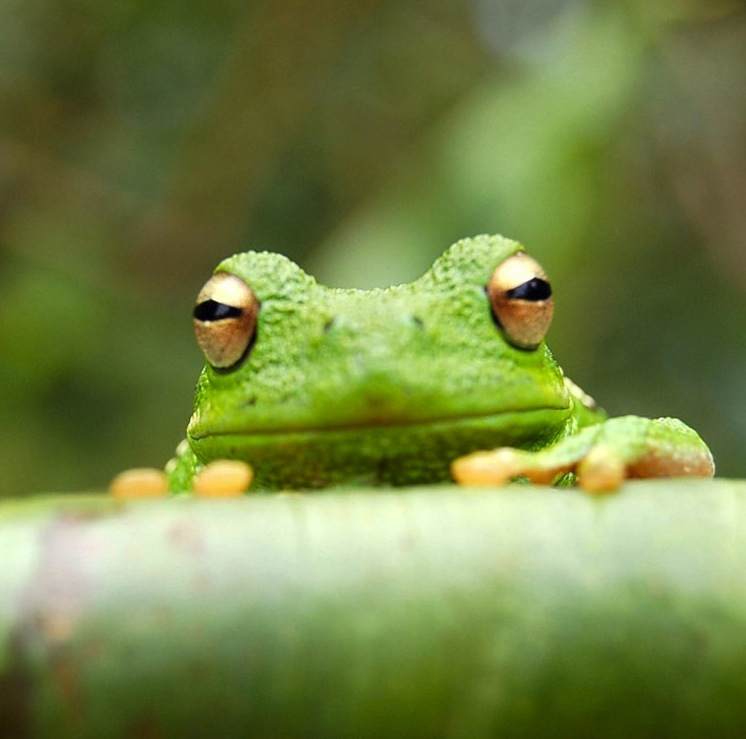
\includegraphics[width=0.3\textwidth]{frog.jpg}
\caption{\label{fig:frog}This frog was uploaded via the file-tree menu.}
\end{figure}

\subsection{Research Questions}

Use the table and tabular environments for basic tables --- see Table~\ref{tab:widgets}, for example. For more information, please see this help article on \href{https://www.overleaf.com/learn/latex/tables}{tables}. 

\begin{table}
\centering
\begin{tabular}{l|r}
Item & Quantity \\\hline
Widgets & 42 \\
Gadgets & 13
\end{tabular}
\caption{\label{tab:widgets}An example table.}
\end{table}

\subsection{How to add Comments and Track Changes}

Comments can be added to your project by highlighting some text and clicking ``Add comment'' in the top right of the editor pane. To view existing comments, click on the Review menu in the toolbar above. To reply to a comment, click on the Reply button in the lower right corner of the comment. You can close the Review pane by clicking its name on the toolbar when you're done reviewing for the time being.

Track changes are available on all our \href{https://www.overleaf.com/user/subscription/plans}{premium plans}, and can be toggled on or off using the option at the top of the Review pane. Track changes allow you to keep track of every change made to the document, along with the person making the change. 

\subsection{How to add Lists}

You can make lists with automatic numbering \dots

\begin{enumerate}
\item Like this,
\item and like this.
\end{enumerate}
\dots or bullet points \dots
\begin{itemize}
\item Like this,
\item and like this.
\end{itemize}

\subsection{How to write Mathematics}

\LaTeX{} is great at typesetting mathematics. Let $X_1, X_2, \ldots, X_n$ be a sequence of independent and identically distributed random variables with $\text{E}[X_i] = \mu$ and $\text{Var}[X_i] = \sigma^2 < \infty$, and let
\[S_n = \frac{X_1 + X_2 + \cdots + X_n}{n}
      = \frac{1}{n}\sum_{i}^{n} X_i\]
denote their mean. Then as $n$ approaches infinity, the random variables $\sqrt{n}(S_n - \mu)$ converge in distribution to a normal $\mathcal{N}(0, \sigma^2)$.


\subsection{How to change the margins and paper size}

Usually the template you're using will have the page margins and paper size set correctly for that use-case. For example, if you're using a journal article template provided by the journal publisher, that template will be formatted according to their requirements. In these cases, it's best not to alter the margins directly.

If however you're using a more general template, such as this one, and would like to alter the margins, a common way to do so is via the geometry package. You can find the geometry package loaded in the preamble at the top of this example file, and if you'd like to learn more about how to adjust the settings, please visit this help article on \href{https://www.overleaf.com/learn/latex/page_size_and_margins}{page size and margins}.

\subsection{How to change the document language and spell check settings}

Overleaf supports many different languages, including multiple different languages within one document. 

To configure the document language, simply edit the option provided to the babel package in the preamble at the top of this example project. To learn more about the different options, please visit this help article on \href{https://www.overleaf.com/learn/latex/International_language_support}{international language support}.

To change the spell check language, simply open the Overleaf menu at the top left of the editor window, scroll down to the spell check setting, and adjust accordingly.


\section {Project Design}

\subsection{Data Collection}

\subsection{Methodology}


\subsubsection{Topic Modeling}
In order to systematically identify semantic themes characterizing user-chatbot interactions, we employed BERTopic, a neural topic modeling approach that leverages transformer-based embeddings to capture latent conversational structure \cite{grootendorst2022bertopic}. After standard preprocessing (stopword removal, lemmatization), we applied BERTopic's three-stage pipeline: (1) UMAP dimensionality reduction, which projects high-dimensional embeddings into lower dimensional space while preserving the semantic structure, (2) HDBSCAN density-based clustering, which identifies semantically coherent clusters, and (3) class-based TF-IDF for topic representation, constraining the model to 20 topics aiming to better interpretability. Topic labels were generated via Mistral-Large (2024) few-shot prompting (for each discovered topic, the model received the top-10 keywords and generated a descriptive label of max 6 words, see Fig. \ref{fig:mistral_prompt}). 
This approach operationalizes the identification of dominant conversational themes, revealing whether chatbots follow users' thematic agendas or introduce divergent content\cite{9031475, chu2025illusionsintimacyemotionalattachment}. 

\begin{figure}
\centering
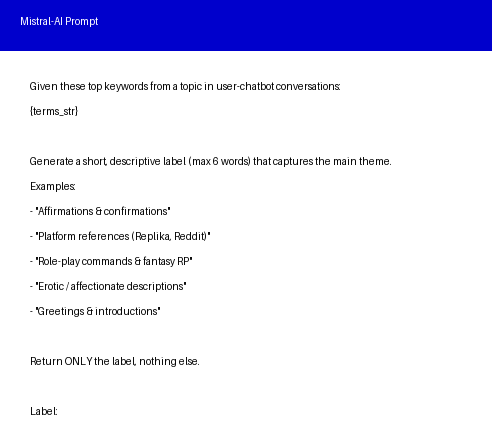
\includegraphics[width=0.4\textwidth]{mistral_prompt.png}
\caption{\label{fig:mistral_prompt}Prompt template used for automatic topic labeling. For each of the 20 topics discovered by BERTopic, Mistral-Large receives the top-10 keywords and generates a descriptive label of maximum 6 words.}
\end{figure}

\subsubsection{Semantic alignment}

To quantify semantic similarity between user and chatbot language, we embed every turn using E5-base \cite{Wang2022TextEB}, chosen for its robust performance on short, conversational text. E5 maps natural language into a 768-dimensional semantic space where cosine similarity reflects meaning overlap. Unlike topic modeling, which assigns text to discrete thematic categories, semantic embeddings capture continuous relatedness, allowing us to measure alignment even when different words express similar concepts (e.g., "happy" vs. "joyful"). To assess global semantic alignment, we computed centroid embeddings for user- and chatbot-generated text separately by averaging all turn-level vectors, then calculated cosine similarity between centroids, a metric ranging from 0 (orthogonal) to 1 (identical semantic space). For visualization, we applied UMAP to project embeddings into 2D space while preserving local semantic structure and revealing distributional patterns. The resulting scatter plot reveals whether user and chatbot expressions occupy overlapping regions (shared semantic space) or form distinct clusters (divergent content). This analysis complements topic modeling by measuring semantic convergence at a continuous, rather than categorical, level: while topic modeling identifies which themes dominate, semantic alignment quantifies how closely the underlying meaning of user and chatbot language converges, even when expressed through different vocabularies.\cite{socioaffective}. 


\section {Results}

\section {Conclusions}

\bibliographystyle{unsrtnat}
\bibliography{sample}

\end{document}